\clearpage

\section{Data vs. MC Comparison in Preselection Region}
\label{sec:yields}

In this section we compare the data and MC samples passing the selection described in Sec.~\ref{sec:eventSelection}
In the following, the MC is reweighted to match the data distribution of number of reconstructed primary vertices.
%{\bf FIXME: UPDATE TO 5.1/fb VTX-REWEIGHTING, CURRENTLY USING OUTDATED FUNCTION}. 
The trigger efficiencies of Sec.~\ref{sec:datasets} are applied. In all plots, the last bin contains the overflow.

We begin by counting the inclusive Z yields. Here we require the presence of two selected leptons without
any additional requirements on jets or \MET. In Fig.~\ref{fig:dilmass} the distribution of dilepton invariant
mass in the ee and $\mu\mu$ channels is displayed. In Table~\ref{table:zyields} the yields for selected dilepton
events in the Z mass window are indicated. Good data vs. MC agreement is observed, within the systematic uncertainties
of integrated luminosity (4.5\%), trigger efficiency (3\%), \zjets\ and \ttbar\ cross sections.

\begin{figure}[hbt]
  \begin{center}
	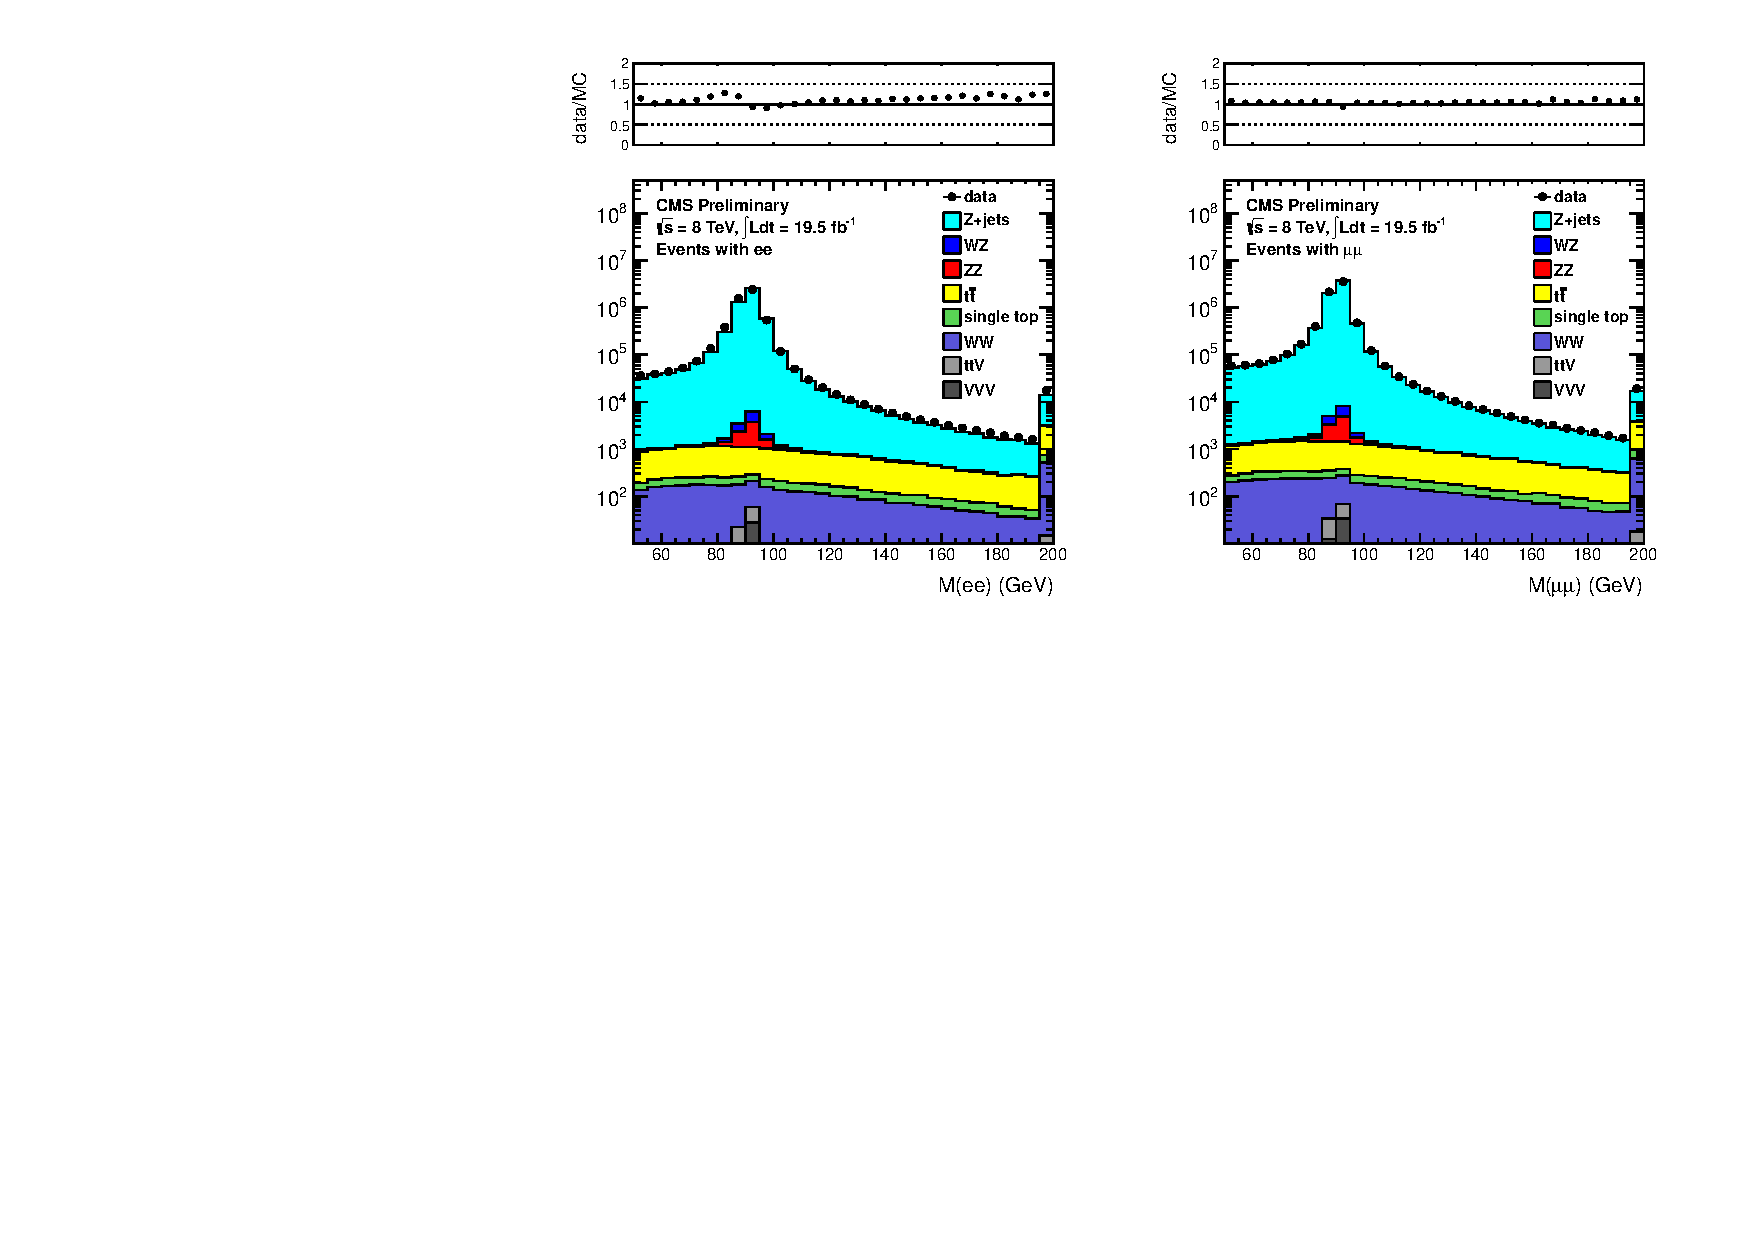
\includegraphics[width=1.0\linewidth]{plots/dilmass_19p5fb.pdf}
	\caption{
	  \label{fig:dilmass}\protect 
	  Dilepton mass distribution for events with two selected leptons
	  in the ee (left) and $\mu\mu$ (right) final states.}

%Loading babies at       : ../output/V00-02-02
%Using selection         : (((((leptype==0 && (ee==1 || isdata==0))||(leptype==1 && (mm==1 || isdata==0)))||(leptype==2 && (em==1||me==1||isdata==0)))&&(csc==0 && hbhe==1 && hcallaser==1 && ecaltp==1 && trkfail==1 && eebadsc==1 && hbhenew==1))&&(lep1.pt()>20.0 && lep2.pt()>20.0))&&(dilmass>15.0)
%Using weight            : weight * 19.5 * trgeff * vtxweight
%Plotting var dilmass flavor ee
%compareDataMC : apply trigeff 1
%MC yield VVV 55.85
%MC yield ttV 110.19
%MC yield WW 3487.10
%MC yield single top 1798.02
%MC yield ttbar 18957.21
%MC yield ZZ 5338.77
%MC yield WZ 5014.99
%MC yield zjets 5404260.14
%MC total yield 5439022.50
%data yield 5.60831e+06
%Plotting var dilmass flavor mm
%compareDataMC : apply trigeff 1
%Warning in <TROOT::Append>: Replacing existing TH1: htemp (Potential memory leak).
%MC yield VVV 69.64
%MC yield ttV 136.01
%MC yield WW 4610.46
%MC yield single top 2321.96
%MC yield ttbar 23578.38
%MC yield ZZ 6981.84
%MC yield WZ 6484.48
%MC yield zjets 7406868.73
%MC total yield 7451051.50
%data yield 7.44536e+06

  \end{center}
\end{figure}


\begin{table}[htb]
\begin{center}
\caption{\label{table:zyields} Data and Monte Carlo yields for events with two selected leptons in the Z mass window. }
\begin{tabular}{lccccc}


%Loading babies at       : ../output/V00-02-02
%Using selection         : ((((((leptype==0 && (ee==1 || isdata==0))||(leptype==1 && (mm==1 || isdata==0)))||(leptype==2 && (em==1||me==1||isdata==0)))&&(csc==0 && hbhe==1 && hcallaser==1 && ecaltp==1 && trkfail==1 && eebadsc==1 && hbhenew==1))&&(lep1.pt()>20.0 && lep2.pt()>20.0))&&(dilmass>15.0))&&(dilmass>81 && dilmass<101)
%Using weight            : weight * 19.5 * trgeff * vtxweight

\hline
\hline
         Sample   &             ee   &       $\mu\mu$   &         e$\mu$   &          total  \\
\hline
         \zjets   &4784691.5 $\pm$ 3465.8   &6575638.5 $\pm$ 3907.6   &2294.1 $\pm$ 74.6   &11362624.1 $\pm$ 5223.7  \\
         \ttbar   &3355.3 $\pm$ 46.1   &4222.2 $\pm$ 49.8   &7624.2 $\pm$ 68.4   &15201.7 $\pm$ 96.3  \\
             WZ   &4342.7 $\pm$ 7.3   &5671.8 $\pm$ 8.0   &114.0 $\pm$ 1.1   &10128.5 $\pm$ 10.9  \\
             ZZ   &4715.2 $\pm$ 9.9   &6192.8 $\pm$ 11.0   & 20.8 $\pm$ 0.3   &10928.8 $\pm$ 14.8  \\
             WW   &614.8 $\pm$ 6.0   &816.3 $\pm$ 6.6   &1417.8 $\pm$ 8.9   &2848.9 $\pm$ 12.7  \\
     single top   &315.3 $\pm$ 11.9   &406.4 $\pm$ 13.0   &701.8 $\pm$ 17.4   &1423.5 $\pm$ 24.8  \\
           \ttV   & 57.4 $\pm$ 1.1   & 70.5 $\pm$ 1.1   & 21.5 $\pm$ 0.7   &149.5 $\pm$ 1.7  \\
            VVV   & 38.9 $\pm$ 0.4   & 49.1 $\pm$ 0.4   &  6.9 $\pm$ 0.2   & 94.9 $\pm$ 0.6  \\
\hline
    total SM MC   &4798131.5 $\pm$ 3466.2   &6593068.0 $\pm$ 3908.0   &12201.2 $\pm$ 103.0   &11403400.7 $\pm$ 5224.7  \\
\hline
           data   &        4906900   &        6552528   &          13141   &       11472569  \\
\hline
\hline

\end{tabular}
\end{center}
\end{table}

\clearpage

We next define the preselection region for the inclusive search using the following requirements:
\begin{itemize}
\item Number of jets $\geq$ 2;
\item Same flavor dileptons (opposite flavor yields will be shown since they are used in data for the FS background estimation);
\item Dilepton invariant mass $81<m_{\ell\ell}<101$ GeV.
\end{itemize}

The dilepton mass distributions in the preselection region of the inclusive search (without the dilepton mass requirement applied) 
for the ee and $\mu\mu$ final states are shown in Figure~\ref{fig:dilmass_2j}. In Table~\ref{table:zyields_2j} the data and MC yields 
in the inclusive preselection region are indicated. Good data vs. MC agreement is observed.


\begin{figure}[hbt]
  \begin{center}
	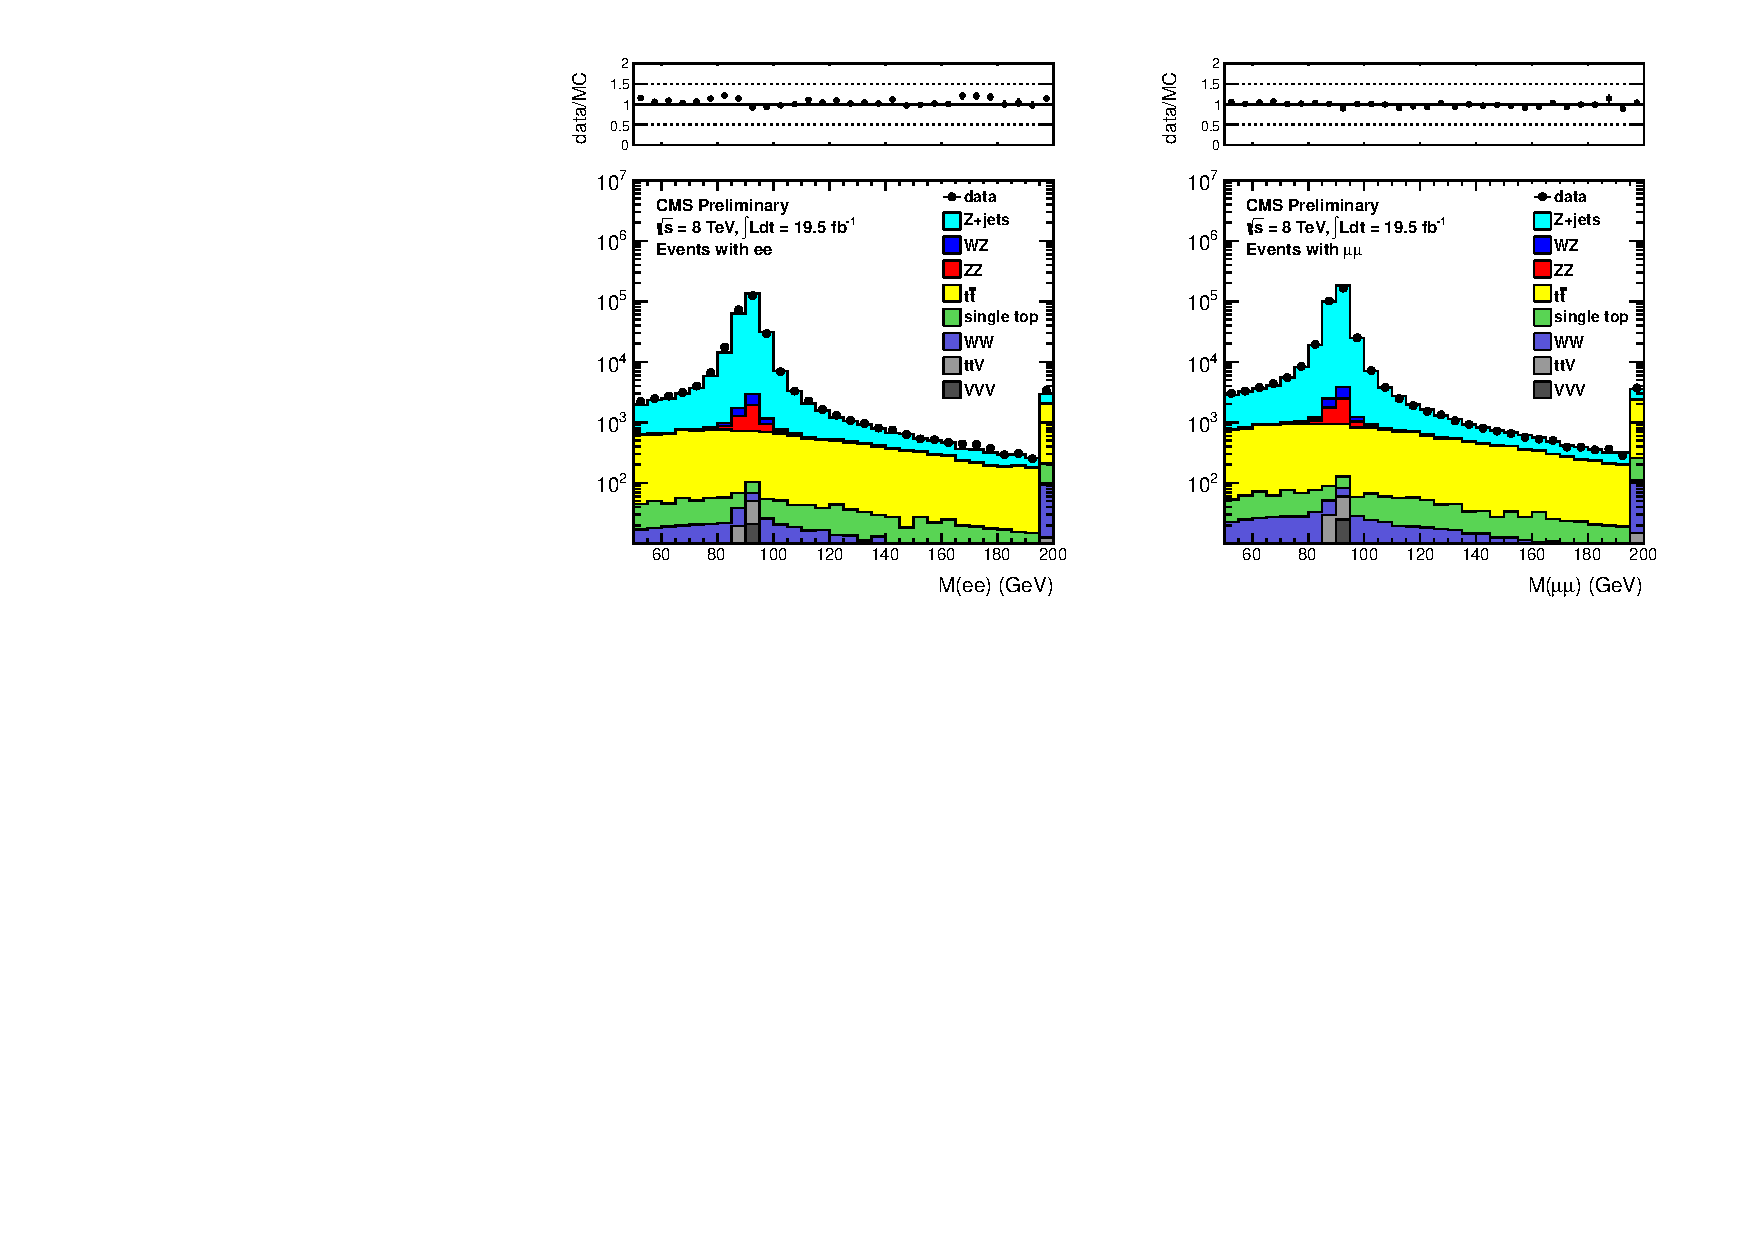
\includegraphics[width=1.0\linewidth]{plots/dilmass_2jets_19p5fb.pdf}
	\caption{
	  \label{fig:dilmass_2j}\protect 
	  Dilepton mass distribution for events in the preselection region of the inclusive search
	  in the ee (left) and $\mu\mu$ (right) final states.}

%Loading babies at       : ../output/V00-02-02
%-------------------------------------
%USING SKIMMED SAMPLES WITH NJETS >= 2
%-------------------------------------

%Using selection         : ((((((leptype==0 && (ee==1 || isdata==0))||(leptype==1 && (mm==1 || isdata==0)))||(leptype==2 && (em==1||me==1||isdata==0)))&&(csc==0 && hbhe==1 && hcallaser==1 && ecaltp==1 && trkfail==1 && eebadsc==1 && hbhenew==1))&&(lep1.pt()>20.0 && lep2.pt()>20.0))&&(dilmass>15.0))&&(njets>=2)
%Using weight            : weight * 19.5 * trgeff * vtxweight
%Plotting var dilmass flavor ee
%compareDataMC : apply trigeff 1
%MC yield VVV 38.82
%MC yield ttV 104.04
%MC yield WW 426.72
%MC yield single top 771.56
%MC yield ttbar 14618.67
%MC yield ZZ 2396.41
%MC yield WZ 2080.63
%MC yield zjets 268774.33
%MC total yield 289211.19
%data yield 291221
%Plotting var dilmass flavor mm
%compareDataMC : apply trigeff 1
%Warning in <TROOT::Append>: Replacing existing TH1: htemp (Potential memory leak).
%MC yield VVV 48.05
%MC yield ttV 129.11
%MC yield WW 549.24
%MC yield single top 980.84
%MC yield ttbar 18175.34
%MC yield ZZ 3092.92
%MC yield WZ 2652.19
%MC yield zjets 358918.68
%MC total yield 384546.38
%data yield 368674

  \end{center}
\end{figure}

\begin{table}[htb]
\begin{center}
\caption{\label{table:zyields_2j} Data and MC yields in the preselection region of the inclusive search.
}
\begin{tabular}{lccccc}

%Loading babies at       : ../output/V00-02-02
%-------------------------------------
%USING SKIMMED SAMPLES WITH NJETS >= 2
%-------------------------------------

%Using selection         : (((((((leptype==0 && (ee==1 || isdata==0))||(leptype==1 && (mm==1 || isdata==0)))||(leptype==2 && (em==1||me==1||isdata==0)))&&(csc==0 && hbhe==1 && hcallaser==1 && ecaltp==1 && trkfail==1 && eebadsc==1 && hbhenew==1))&&(lep1.pt()>20.0 && lep2.pt()>20.0))&&(dilmass>15.0))&&(njets>=2))&&(dilmass>81 && dilmass<101)
%Using weight            : weight * 19.5 * trgeff * vtxweight

\hline
\hline
         Sample   &             ee   &       $\mu\mu$   &         e$\mu$   &          total  \\
\hline
         \zjets   &237881.9 $\pm$ 762.8   &317954.1 $\pm$ 848.2   &121.7 $\pm$ 17.1   &555957.7 $\pm$ 1140.9  \\
          ttbar   &2597.5 $\pm$ 40.5   &3268.0 $\pm$ 43.8   &5926.8 $\pm$ 60.2   &11792.4 $\pm$ 84.7  \\
             WZ   &1814.8 $\pm$ 4.8   &2329.0 $\pm$ 5.3   & 22.8 $\pm$ 0.5   &4166.6 $\pm$ 7.1  \\
             ZZ   &2123.3 $\pm$ 7.0   &2750.6 $\pm$ 7.7   &  4.8 $\pm$ 0.2   &4878.8 $\pm$ 10.4  \\
             WW   & 69.6 $\pm$ 2.0   & 90.3 $\pm$ 2.2   &161.1 $\pm$ 3.0   &321.0 $\pm$ 4.2  \\
     single top   &128.6 $\pm$ 7.6   &155.3 $\pm$ 8.0   &280.1 $\pm$ 11.0   &564.0 $\pm$ 15.6  \\
           \ttV   & 55.2 $\pm$ 1.0   & 68.0 $\pm$ 1.1   & 20.0 $\pm$ 0.6   &143.2 $\pm$ 1.6  \\
            VVV   & 28.7 $\pm$ 0.3   & 36.1 $\pm$ 0.3   &  3.5 $\pm$ 0.1   & 68.3 $\pm$ 0.5  \\
\hline
    total SM MC   &244699.8 $\pm$ 764.0   &326651.4 $\pm$ 849.5   &6540.8 $\pm$ 63.6   &577892.0 $\pm$ 1144.2  \\
\hline
           data   &         243387   &         310368   &           6416   &         560171  \\
\hline
\hline



\end{tabular}
\end{center}
\end{table}


\clearpage

We next define the preselection region for the targeted search by adding the following requirements:
\begin{itemize}
\item Veto events containing a b-tagged jet;
\item Dijet invariant mass $70<m_{jj}<110$ GeV;
\item Veto events containing a third selected lepton (electron or muon) with \pt $>$ 10 GeV; 
\end{itemize}

The rejection of events with a b-tagged jet strongly suppresses the \ttbar\ background, which is the dominant background in the inclusive search
after requiring large \MET. The requirement that the jet pair is consistent with originating from W/Z decay is motivated by the fact that we are 
searching for signatures producing V(jj)Z($\ell\ell$)+\MET; this requirement suppresses the \zjets\ and \ttbar\ backgrounds. The veto of events
containting a third electron or muon suppresses the WZ background, and also serves to make this analyis exclusive with respect to searches in
the trilepton final state.

The dilepton mass distributions in the preselection region of the targeted search (without the dilepton mass requirement applied) 
for the ee and $\mu\mu$ final states are shown in Figure~\ref{fig:dilmass_2j_targeted}. In Table~\ref{table:zyields_2j_targeted} 
the data and MC yields in the preselection region are indicated. Good data vs. MC agreement is observed.
We also show the distribution of dijet mass in the targeted preselection (with the requirement on this quantity removed) in Fig.~\ref{fig:mjj},
which demonstrates that the MC does a reasonable job of modeling this quantity.

%-------------------------------------
% veto b-jets with CSV MEDIUM 
%-------------------------------------

\begin{figure}[hbt]
  \begin{center}
	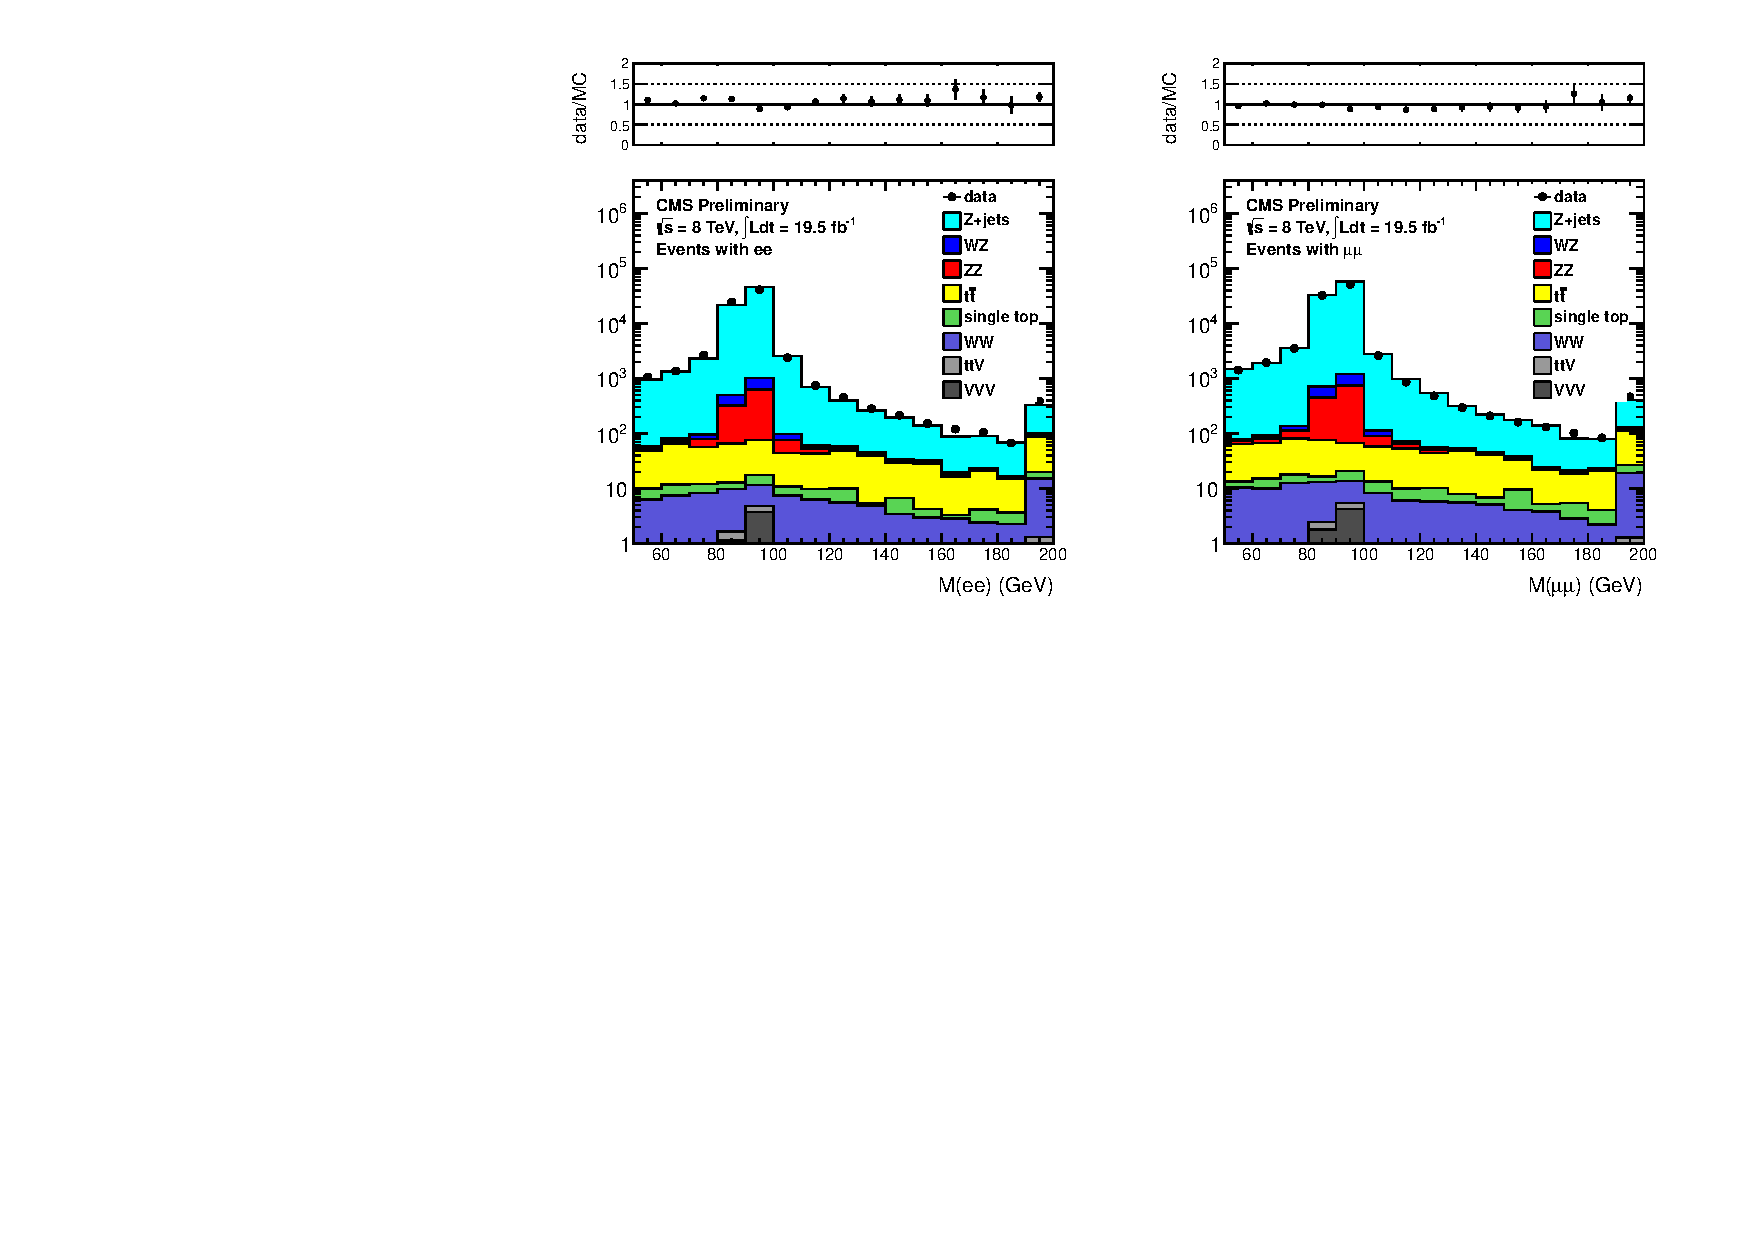
\includegraphics[width=1.0\linewidth]{plots/dilmass_targeted_19p5fb.pdf}
	\caption{
	  \label{fig:dilmass_2j_targeted}\protect 
	  Dilepton mass distribution for events in the preselection region of the targeted search
	  in the ee (left) and $\mu\mu$ (right) final states.}

%Loading babies at       : ../output/V00-02-02
%-------------------------------------
%USING SKIMMED SAMPLES WITH NJETS >= 2
%-------------------------------------

%Using selection         : (((((((((leptype==0 && (ee==1 || isdata==0))||(leptype==1 && (mm==1 || isdata==0)))||(leptype==2 && (em==1||me==1||isdata==0)))&&(csc==0 && hbhe==1 && hcallaser==1 && ecaltp==1 && trkfail==1 && eebadsc==1 && hbhenew==1))&&(lep1.pt()>20.0 && lep2.pt()>20.0))&&(dilmass>15.0))&&(njets>=2))&&(nbcsvm==0))&&(mjj>70.0 && mjj<110.0))&&(nlep==2)
%Using weight            : weight * 19.5 * trgeff * vtxweight
%Plotting var dilmass flavor ee
%compareDataMC : apply trigeff 1
%MC yield VVV 7.33
%MC yield ttV 3.58
%MC yield WW 85.67
%MC yield single top 45.33
%MC yield ttbar 543.24
%MC yield ZZ 918.93
%MC yield WZ 630.62
%MC yield zjets 74954.58
%MC total yield 77189.27
%data yield 75429
%Plotting var dilmass flavor mm
%compareDataMC : apply trigeff 1
%Warning in <TROOT::Append>: Replacing existing TH1: htemp (Potential memory leak).
%MC yield VVV 9.03
%MC yield ttV 3.68
%MC yield WW 110.10
%MC yield single top 60.55
%MC yield ttbar 623.36
%MC yield ZZ 1182.18
%MC yield WZ 814.62
%MC yield zjets 101116.68
%MC total yield 103920.20
%data yield 96236

  \end{center}
\end{figure}

\begin{table}[htb]
\begin{center}
\caption{\label{table:zyields_2j_targeted} Data and MC yields in the preselection region of the targeted search.
}
\begin{tabular}{lccccc}

%Loading babies at       : ../output/V00-02-02
%-------------------------------------
%USING SKIMMED SAMPLES WITH NJETS >= 2
%-------------------------------------

%Using selection         : ((((((((((leptype==0 && (ee==1 || isdata==0))||(leptype==1 && (mm==1 || isdata==0)))||(leptype==2 && (em==1||me==1||isdata==0)))&&(csc==0 && hbhe==1 && hcallaser==1 && ecaltp==1 && trkfail==1 && eebadsc==1 && hbhenew==1))&&(lep1.pt()>20.0 && lep2.pt()>20.0))&&(dilmass>15.0))&&(njets>=2))&&(nbcsvm==0))&&(mjj>70.0 && mjj<110.0))&&(nlep==2))&&(dilmass>81 && dilmass<101)
%Using weight            : weight * 19.5 * trgeff * vtxweight

\hline
\hline
         Sample   &             ee   &       $\mu\mu$   &         e$\mu$   &          total  \\
\hline
         \zjets   &66277.1 $\pm$ 401.2   &89182.1 $\pm$ 447.5   & 26.8 $\pm$ 8.1   &155486.1 $\pm$ 601.1  \\
         \ttbar   &108.2 $\pm$ 8.3   &106.6 $\pm$ 7.8   &223.6 $\pm$ 11.7   &438.4 $\pm$ 16.3  \\
             WZ   &553.1 $\pm$ 2.7   &718.0 $\pm$ 3.0   &  3.6 $\pm$ 0.2   &1274.7 $\pm$ 4.0  \\
             ZZ   &816.3 $\pm$ 4.4   &1052.1 $\pm$ 4.8   &  0.9 $\pm$ 0.1   &1869.3 $\pm$ 6.6  \\
             WW   & 14.6 $\pm$ 0.9   & 18.3 $\pm$ 1.0   & 34.4 $\pm$ 1.4   & 67.3 $\pm$ 1.9  \\
     single top   &  9.5 $\pm$ 2.1   & 10.9 $\pm$ 2.1   & 18.6 $\pm$ 2.8   & 39.0 $\pm$ 4.1  \\
           \ttV   &  1.6 $\pm$ 0.2   &  1.8 $\pm$ 0.2   &  0.8 $\pm$ 0.1   &  4.2 $\pm$ 0.3  \\
            VVV   &  4.8 $\pm$ 0.1   &  6.1 $\pm$ 0.1   &  0.9 $\pm$ 0.1   & 11.8 $\pm$ 0.2  \\
\hline
    total SM MC   &67785.3 $\pm$ 401.3   &91095.8 $\pm$ 447.6   &309.7 $\pm$ 14.6   &159190.9 $\pm$ 601.3  \\
\hline
           data   &          65376   &          83864   &            312   &         149552  \\
\hline
\hline

\end{tabular}
\end{center}
\end{table}



\begin{comment}

%-------------------------------------
% veto b-jets with CSV LOOSE 
%-------------------------------------

\begin{figure}[hbt]
  \begin{center}
	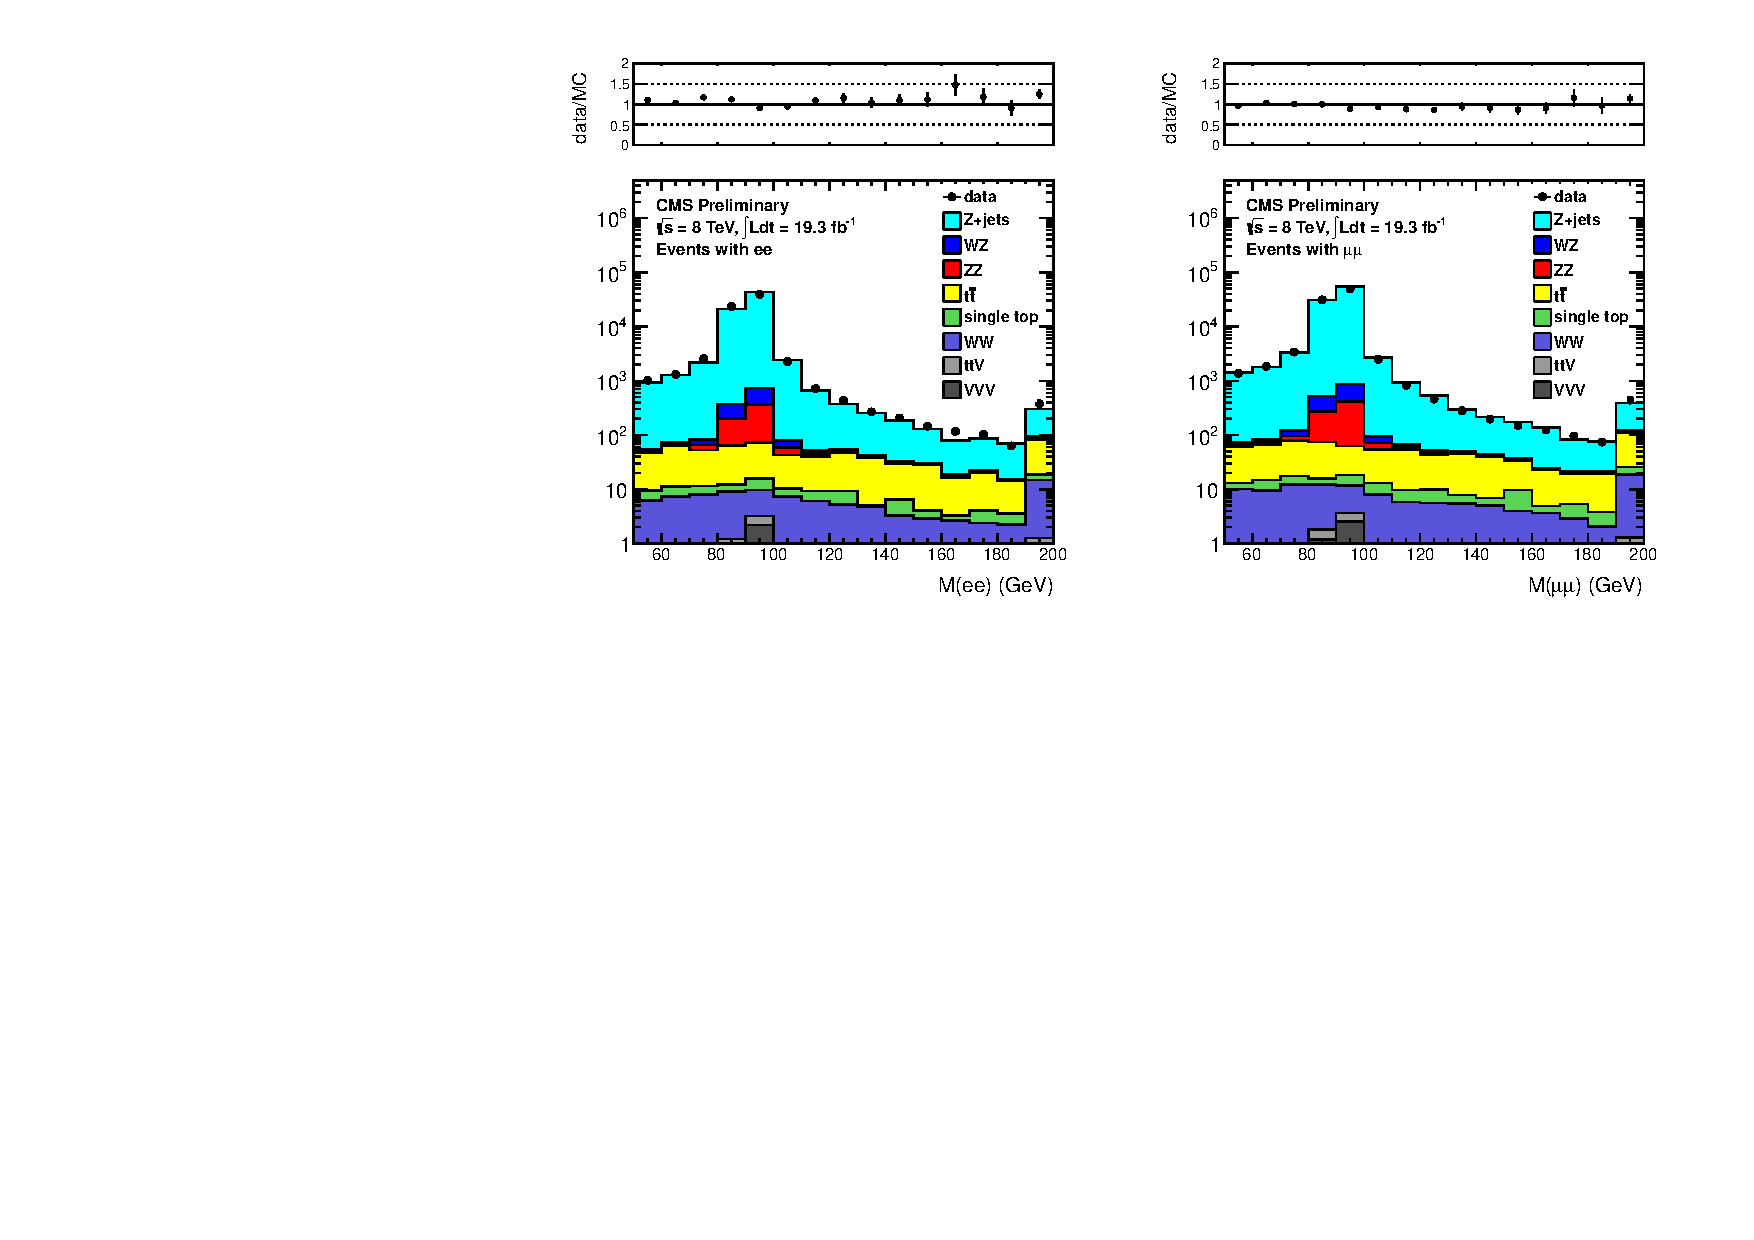
\includegraphics[width=1.0\linewidth]{plots/dilmass_targeted_19fb.pdf}
	\caption{
	  \label{fig:dilmass_2j_targeted}\protect 
	  Dilepton mass distribution for events in the preselection region of the targeted search
	  in the ee (left) and $\mu\mu$ (right) final states.}

%Loading babies at       : ../output/V00-01-04
%-------------------------------------
%USING SKIMMED SAMPLES WITH NJETS >= 2
%-------------------------------------

%Using selection         : ((((((((isdata==0 || (run<197556 || run>198913))&&(((leptype==0 && (ee==1 || isdata==0))||(leptype==1 && (mm==1 || isdata==0)))||(leptype==2 && (em==1||me==1||isdata==0))))&&(csc==0 && hbhe==1 && hcallaser==1 && ecaltp==1 && trkfail==1 && eebadsc==1 && hbhenew==1))&&(lep1.pt()>20.0 && lep2.pt()>20.0))&&(dilmass>15.0))&&(njets>=2))&&(nbcsvl==0))&&(mjj>70.0 && mjj<110.0))&&(nlep==2)
%Using weight            : weight * 9.2 * trgeff * vtxweight
%Plotting var dilmass flavor ee
%compareDataMC : apply trigeff 1
%MC yield VVV 1.69
%MC yield ttV 0.71
%MC yield WW 29.99
%MC yield single top 10.71
%MC yield ttbar 98.96
%MC yield ZZ 160.28
%MC yield WZ 201.63
%SCALING ZJETS BY 111/946
%MC yield zjets 26365.25
%MC total yield 26869.22
%data yield 24722
%Plotting var dilmass flavor mm
%compareDataMC : apply trigeff 1
%Warning in <TROOT::Append>: Replacing existing TH1: htemp (Potential memory leak).
%MC yield VVV 2.05
%MC yield ttV 0.70
%MC yield WW 38.74
%MC yield single top 13.48
%MC yield ttbar 104.95
%MC yield ZZ 206.22
%MC yield WZ 262.27
%SCALING ZJETS BY 111/946
%MC yield zjets 35489.85
%MC total yield 36118.25
%data yield 32393

  \end{center}
\end{figure}

\begin{table}[htb]
\begin{center}
\caption{\label{table:zyields_2j_targeted} Data and MC yields in the preselection region of the inclusive search.
}
\begin{tabular}{lccccc}
\hline
\hline
         Sample   &           ee   &       $\mu\mu$   &         e$\mu$   &            total  \\
\hline

%Loading babies at       : ../output/V00-01-04
%-------------------------------------
%USING SKIMMED SAMPLES WITH NJETS >= 2
%-------------------------------------

%Using selection         : (((((((((isdata==0 || (run<197556 || run>198913))&&(((leptype==0 && (ee==1 || isdata==0))||(leptype==1 && (mm==1 || isdata==0)))||(leptype==2 && (em==1||me==1||isdata==0))))&&(csc==0 && hbhe==1 && hcallaser==1 && ecaltp==1 && trkfail==1 && eebadsc==1 && hbhenew==1))&&(lep1.pt()>20.0 && lep2.pt()>20.0))&&(dilmass>15.0))&&(njets>=2))&&(nbcsvl==0))&&(mjj>70.0 && mjj<110.0))&&(nlep==2))&&(dilmass>81 && dilmass<101)
%Using weight            : weight * 9.2 * trgeff * vtxweight

\hline
         Sample   &           $ee$   &       $\mu\mu$   &         $e\mu$   &            tot  \\
\hline
SCALING ZJETS BY 111/946
          zjets   &23338.4 $\pm$ 164.1   &31251.5 $\pm$ 182.6   &  8.9 $\pm$ 3.1   &54598.8 $\pm$ 245.5  \\
             WZ   &176.4 $\pm$ 1.1   &231.1 $\pm$ 1.2   &  1.1 $\pm$ 0.1   &408.7 $\pm$ 1.6  \\
             ZZ   &142.3 $\pm$ 0.9   &183.2 $\pm$ 1.0   &  0.1 $\pm$ 0.0   &325.6 $\pm$ 1.4  \\
          ttbar   & 20.6 $\pm$ 2.5   & 15.5 $\pm$ 2.1   & 38.1 $\pm$ 3.4   & 74.2 $\pm$ 4.7  \\
     single top   &  2.3 $\pm$ 0.7   &  2.9 $\pm$ 0.7   &  4.5 $\pm$ 1.0   &  9.6 $\pm$ 1.4  \\
             WW   &  5.0 $\pm$ 0.4   &  6.8 $\pm$ 0.4   & 12.3 $\pm$ 0.6   & 24.2 $\pm$ 0.8  \\
            ttV   &  0.3 $\pm$ 0.1   &  0.3 $\pm$ 0.1   &  0.2 $\pm$ 0.0   &  0.8 $\pm$ 0.1  \\
            VVV   &  0.9 $\pm$ 0.0   &  1.1 $\pm$ 0.0   &  0.3 $\pm$ 0.0   &  2.3 $\pm$ 0.1  \\
\hline
      tot SM MC   &23686.1 $\pm$ 164.1   &31692.4 $\pm$ 182.6   & 65.7 $\pm$ 4.7   &55444.2 $\pm$ 245.5  \\
\hline
           data   &          21529   &          28265   &             53   &          49847  \\
\hline
\hline

\end{tabular}
\end{center}
\end{table}

\end{comment}


\clearpage

\begin{figure}[hbt]
  \begin{center}
	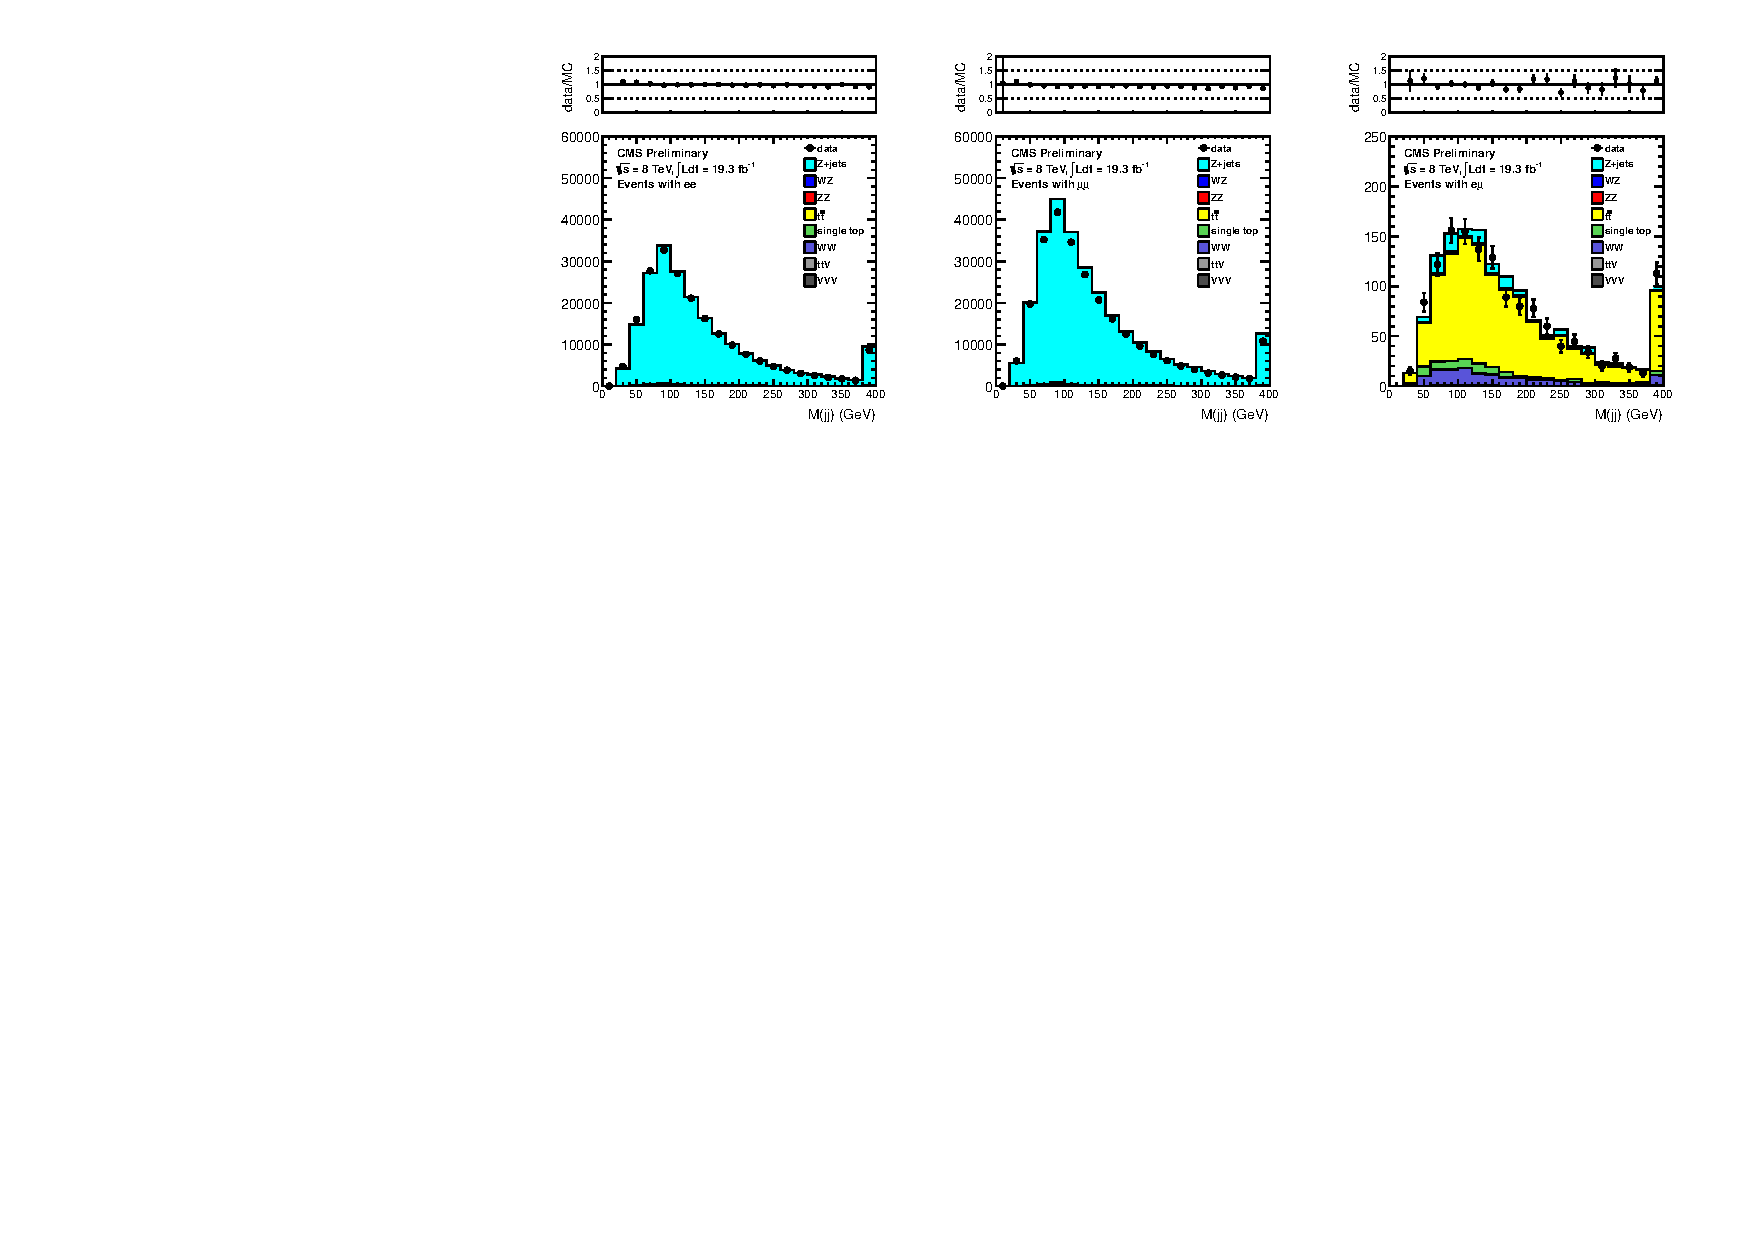
\includegraphics[width=1.0\linewidth]{plots/mjj_targeted_19fb.pdf}
	\caption{
	  \label{fig:mjj}\protect 
Distributions of dijet mass for the targeted preselection in the ee (left), $\mu\mu$ (middle) and e$\mu$ (right) final state.
}                   
  \end{center}
\end{figure}



%Loading babies at       : ../output/V00-02-00
%-------------------------------------
%USING SKIMMED SAMPLES WITH NJETS >= 2
%-------------------------------------

%Using selection         : ((((((((isdata==0 || (run<197556 || run>198913))&&(((leptype==0 && (ee==1 || isdata==0))||(leptype==1 && (mm==1 || isdata==0)))||(leptype==2 && (em==1||me==1||isdata==0))))&&(csc==0 && hbhe==1 && hcallaser==1 && ecaltp==1 && trkfail==1 && eebadsc==1 && hbhenew==1))&&(lep1.pt()>20.0 && lep2.pt()>20.0))&&(dilmass>15.0))&&(njets>=2))&&(nbcsvm==0))&&(nlep==2))&&(dilmass>81 && dilmass<101)
%Using weight            : weight * 19.3 * trgeff * vtxweight
%Plotting var mjj flavor ee
%compareDataMC : apply trigeff 1
%MC yield VVV 12.21
%MC yield ttV 7.75
%MC yield WW 63.50
%MC yield single top 33.64
%MC yield ttbar 435.66
%MC yield ZZ 859.71
%MC yield WZ 1520.22
%SCALING ZJETS BY 111/946
%MC yield zjets 209451.48
%MC total yield 212384.17
%data yield 209905
%Plotting var mjj flavor mm
%compareDataMC : apply trigeff 1
%Warning in <TROOT::Append>: Replacing existing TH1: htemp (Potential memory leak).
%MC yield VVV 15.69
%MC yield ttV 9.57
%MC yield WW 81.36
%MC yield single top 42.28
%MC yield ttbar 539.62
%MC yield ZZ 1113.63
%MC yield WZ 1955.65
%SCALING ZJETS BY 111/946
%MC yield zjets 281080.79
%MC total yield 284838.59
%data yield 266373
%Plotting var mjj flavor em
%compareDataMC : apply trigeff 1
%Warning in <TROOT::Append>: Replacing existing TH1: htemp (Potential memory leak).
%MC yield VVV 2.59
%MC yield ttV 3.22
%MC yield WW 143.37
%MC yield single top 77.11
%MC yield ttbar 1087.65
%MC yield ZZ 1.32
%MC yield WZ 15.18
%SCALING ZJETS BY 111/946
%MC yield zjets 112.51
%MC total yield 1442.95
%data yield 1417

